\documentclass[11pt]{extarticle}
\usepackage[spanish,english]{babel}
\usepackage[utf8]{inputenc}
\usepackage[letterpaper,margin=2.54cm]{geometry}
\usepackage{graphicx}
\usepackage[spanish]{babel}
\usepackage{titlesec}
\usepackage{tocloft}%
\graphicspath{/Users/mijatola/Documents/Tesis}
\selectlanguage{spanish}
\let \savenumberline \numberline
\def \numberline#1{\savenumberline{#1.}}

\date{}
\author{}

\begin{document}

\title{
    \textbf{
      \Large{UNIVERSIDAD MAYOR DE SAN ANDRES}\\
      \normalsize{
        FACULTAD DE CIENCIAS PURAS Y NATURALES\\
        CARRERA DE INFORMATICA\\
      }
      \hfill \break
      
\includegraphics[width=5cm,height=10cm]{umsa}
      \break
      \begin{large}
        PERFIL DE TESIS DE GRADO
        \break
        \break
        GENERADOR DE GRAFOS ALEATORIOS PARA CASOS DE PRUEBA
      \end{large}
      \break
      \break
      \small{
        Proyecto de Grado para obtener el Título de Licenciatura en Informática \break
        Mención Ingeniería de Sistemas Informáticos\break
      }
      \break
      \large {
        POR: CARLOS MIJAEL TOLA APAZA\\
        TUTOR: LIC. JORGE TERAN
      }
      \break
      \small {
        LA PAZ - BOLIVIA \break
        Noviembre, 2021
      }
    }
}

\maketitle
\selectlanguage{spanish}
\tableofcontents
\newpage

\titleformat*{\section}{\normalsize\bfseries\MakeUppercase}
\titleformat*{\subsection}{\normalsize\bfseries\MakeUppercase}
\titlelabel{\thetitle.\quad}

\newcommand\justificacion{Justificaci\'on }
\newcommand\guion{\item[-]}

\renewcommand{\labelenumii}{\arabic{enumi}.\arabic{enumii}}
\renewcommand{\labelenumiii}{\arabic{enumi}.\arabic{enumii}.\arabic{enumiii}}
\renewcommand{\labelenumiv}{\arabic{enumi}.\arabic{enumii}.\arabic{enumiii}.\arabic{enumiv}}

\section{Introduccion} 
El uso generalizado de grafos aleatorios se ha destacado en el contexto de las 
aplicaciones de bases de datos y análisis de algoritmos durante 
varios años. Esto se debe a que tales estructuras de datos resultan ser muy útiles 
en muchas  aplicaciones, desde el análisis de redes complejas hasta el estudio de 
algoritmos aleatorios. El problema es que generar estos grafos aleatorios no es una 
tarea fácil. Y es ahí donde entramos, con un modelo generador de grafos aleatorios que 
generan grafos aleatorios en un tiempo eficiente. Debido a que en Teoría de Grafos 
existe una infinidad de tipos de grafos, nos enfocaremos simplemente en un conjunto 
de grafos que son: Grafos directos acíclicos (DAG), Grafos Bipartitos, Grafos completos,
 Grafos no dirigidos conexos y no conexos, y árboles.

\section{Antecedentes}
Se conocen muchos modelos de grafos aleatorios, que reflejan los diversos tipos de redes
complejas que se encuentran en diferentes áreas. En un contexto matemático, el grafo aleatorio 
se refiere casi exclusivamente al modelo de grafo aleatorio de Erdős-Rényi. 
Se ha argumentado correctamente que los grafos aleatorios de Erdős-Rényi
generalmente no son representativos de los grafos de la vida real, como las redes de comunicación,
las redes sociales o las estructuras moleculares, que exhiben distribuciones de grados específicas y propiedades 
resultantes. Sin embargo, si los grafos de la vida real difieren significativamente de los grafos 
de Erdős-Rényi, todavía se necesitan modelos de Erdős-Rényi para caracterizar estas diferencias y cuantificar 
su importancia. La generación de grafos aleatorios con restricciones prescritas generalmente requiere una maquinaria diferente 
y más compleja. El método predominante es el uso de la mezcla de cadenas de Markov, para la generación de estructuras 
de marca como grafos bipartitos de transacciones y elementos con restricciones de grado prescritas.\\

Al respecto de las investigaciones relacionadas con el tema podemos destacar las siguientes:

\begin{itemize}
  \item \textbf{Titulo:} Desempeño asintótico de algoritmos secuenciales
  en grafos aleatorios - Tesis presentada para optar al título de Doctor.\\
  \textbf{Autor:} Lic. Manuel Sáenz \\
  \textbf{A\~no:} 2019\\
  \textbf{Institucion:} Universidad de Buenos Aires\\
\end{itemize}

\begin{itemize}
  \item \textbf{Titulo:} Generación rápida de gráficos aleatorios\\
  \textbf{Autor:} Sadegh Heyrani, Nobari Xuesong Lu \\
  \textbf{A\~no:} 2011\\
  \textbf{Institucion:} Universidad Nacional de Singapore\\
\end{itemize}

\begin{itemize}
  \item \textbf{Titulo:} Implementacion de un generador de topologias aleatorias en emulador de red mininet.\\
  \textbf{Autor:} Rosa Alejandra García Grisales, Juan Carlos Agudelo Calderón\\
  \textbf{A\~no:} 2015\\
  \textbf{Institucion:} Universidad Católica De Pereira\\
\end{itemize}

\begin{itemize}
  \item \textbf{Titulo:} Modelado de grafos aleatorios: una revisión de los conceptos\\
  \textbf{Autor:} Mikhail Drobyshevskiy, Denis Turdakov\\
  \textbf{A\~no:} 2019\\
  \textbf{Institucion:} Instituto de Física y Tecnología de Moscú\\
\end{itemize}



\section{Planteamiento del problema}
  Como ya se hab\'ia sugerido anteriormente, el modelado de grafos juega un rol 
  importante en el analisis de redes complejas. Nos ayudan a entender, controlar
  predecir fenomenos que pueden ocurrir en redes sociales, redes biologicas, internet
  y muchos mas. Modelar estos grafos manualmente para cada aplicacion podria requerir
  demasiado tiempo y esfuerzo.
  \subsection{Problema central}
    ¿C\'omo podriamos modelar estos grafos o topologias en un tiempo eficiente?
  \subsection{Problemas secundarios}
    \begin{itemize}
      \guion Construir un grafo completo es NP. 
      \guion Como comprobar si el model fue generado en un tiempo eficiente.
    \end{itemize}
\section{Hip\'otesis}
  El metodo propuesto para la generacion de grafos de forma aleatorio 
  tendro un grado mayor de eficiencia con respecto a los metodos
  usados anteriormente por otras investigaciones en un 95\%.

\section{Definicion de objectivos}
  \subsection{Objetivo general}
  Implementar un modelo generador de grafos aleatorios para usarlos como casos de prueba.
  \subsection{Objetivos secundarios}
      \begin{itemize}
        \guion Analizar y diseñar un modelo generador de grafos aleatorios para: Grafos directos acíclicos (DAG), Grafos Bipartitos, Grafos completos, Grafos no dirigidos conexos y no conexos, y árboles.
        \guion Verificar que los tiempos al generar los grafos sean eficientes experimentalmente.
        \guion Verificar que el generador de grafos sea eficiente según su complejidad algorítmica.
      \end{itemize}
\section{\justificacion}
  \subsection{\justificacion econ\'omica}
    Modelar y/o generar grafos de manera eficiente significa que se reduciran los costos de energia y se
    eliminara el tiempo invertido en el modelado de las topografias. 
  \subsection{\justificacion social}
    El impacto que tienen las redes sociales hoy en d\'ia en la sociedad es bastante notorio,
    estas redes sociales siempre esta a la mejora de sus algorimos debido al creciemiento en referencia a usuarios.
    Para esto es necesario investigar y probar dichos algoritmos en topologias aleatorias.
  \subsection{\justificacion cient\'fica}
    El presente trabajo combinara tecnicas algor\'itmicas, mascaras de bits utilizando tecnicas
    matematicas de tal manera que el modelado de las topologias sea eficiente,
    esto se puede verificar usando notaciones de complejidad algor\'itmicas.
\section{Alcances y limites}
  \subsection{Alcances}
    \begin{itemize}
      \guion El presente trabajo diseñara un modelo generador de grafos aleatorios
            para DAGs, Grafos bipartitos, Grafos completos, Grafos no dirigidos
            conexos y no conexos, y arboles de manera eficiente.
      \end{itemize}
  \subsection{L\'imites}
    El siguiente trabajo no contempla los siguientes aspectos
    \begin{itemize}
      \guion Los grafos que no esten contemplados en los alcances,
             ya que probablemente sean tipos de grafos NP (Grafos Planares).
    \end{itemize}
\section{Metodolog\'ia}
  Para el desarrollo del presente proyecto se utilizara un 
  \textbf{Metodo de investigacion experimental} para cumplir con los 
    objectivos propuestos para el modelo de generador de grafos aleatorios. 
    Esta se dividirar en las siguientes etapas.
    \begin{itemize}
      \item Recopilacion de informacion.
      \item Elaboracion del Modelo generador de grafos aleatorios.
      \item Pruebas de funcionamiento y/o presentación de mejoras para el modelo.
      \item Comparaciones y analisis de los datos.
      \item Conclusiones.
    \end{itemize}
    
    La primera etapa se recopilara la informacion necesaria y
    se estudiara temas relacionadas al mismo.\hfill\break

    La segunda etapa se realizara el Modelo generado de grafos tomando
    encuenta los alcances y limites. \hfill\break

    La tercera etapa se verificara la funcionalidad del modelo.
    \hfill\break

    En la cuarta etapa se analizaran los datos y se los comparara con 
    otros modelos.
    \hfill\break

    En la ultima etapa, se presentaran los resultados finales, las
    conclusienes y recomendaciones con respecto al proyecto

\section{Bibliograf\'ia}
  Manuel Zaens. (2019). Desempeño asintotico de algoritmos secuenciales en grafos aleatorios. 2019, de Universidad de Buenos Aires Sitio web:\hfill\break http://cms.dm.uba.ar/academico/carreras/doctorado/Tesis\_Saenz\_corregida(1).pdf \hfill \break
  \break
  Sadegh Heyrani, Nobari Xuesong Lu. (2011). Generaci\'on r\'apida de gr\'aficos aleatorios. 2019, de Universidad Nacional de Singapore Sitio web: https://www.cs.au.dk/~karras/rg.pdf
  \break
  \break
  Rosa Alejandra Garc\'ia Grisales, Juan Carlos Agudelo Calder\'on. (2015). Implementacion de un generador de topologias aleatorias en emulador de red mininet.. 2019, de Universidad Cat\'olica De Pereira Sitio web: https://repositorio.ucp.edu.co/bitstream/10785/3678/1/CDMIST122.pdf
  \break
  \break
  Mikhail Drobyshevskiy, Denis Turdakov. (2019). Modelado de grafos aleatorios: una revis\'ion de los conceptos. 2019, de Mikhail Drobyshevskiy, Denis Turdakov Sitio web:\hfill\break https://dl.acm.org/doi/pdf/10.1145/3369782
\section{Anexos}
\subsection{Cronograma de avance}
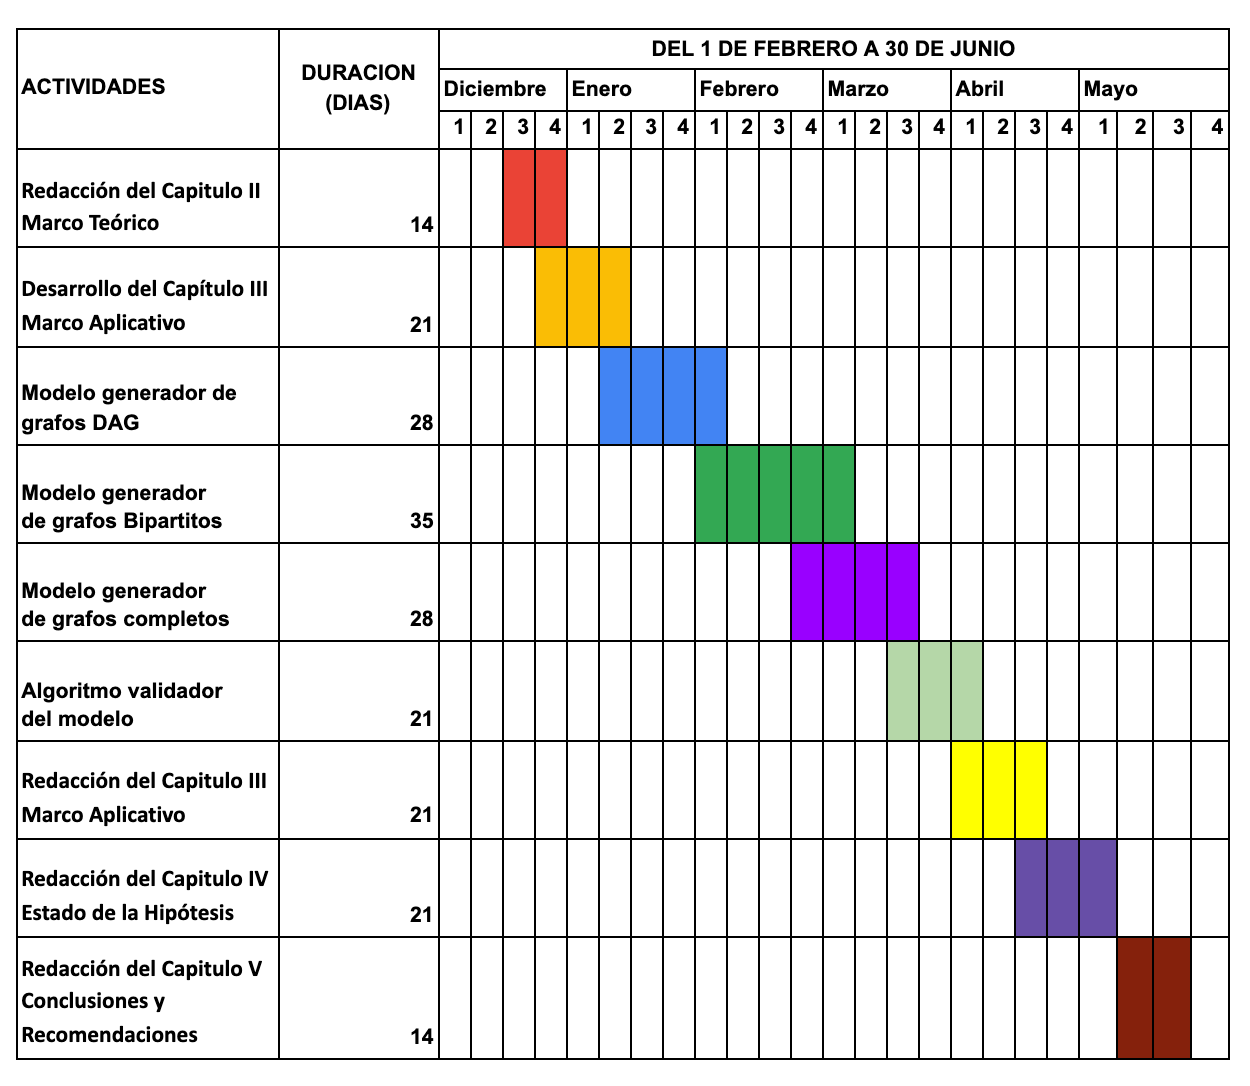
\includegraphics[width=18cm,height=15cm]{calendario.png}
\subsection{Indice de trabajo}
  \begin{enumerate}
    \item CAPÍTULO 1: MARCO REFERENCIAL
    \begin{enumerate}
      \item Introduccion
      \item Antecedentes
      \item Planteamiento del problema
        \begin{enumerate}
          \item Problema central
          \item Problemas secundarios
        \end{enumerate}
      \item Objetivo
        \begin{enumerate}
          \item Objetivo principal
          \item objectivos secundarios
        \end{enumerate}
      \item Hip\'otesis
      \item \justificacion
        \begin{enumerate}
          \item \justificacion econ\'omica
          \item \justificacion social
          \item \justificacion cient\'ifica
        \end{enumerate}
      \item Alcances y L\'imites
        \begin{enumerate}
          \item Alcances
          \item L\'imites
        \end{enumerate}
      \item Metodolog\'ia
    \end{enumerate}
    \item CAPITULO 2: MARCO TEORICO
      \begin{enumerate}
        \item Mascaras de bits
        \begin{enumerate}
          \item Operaciones con mascaras de bits
        \end{enumerate}
        \item Programac\'ion din\'amica (DP)
        \begin{enumerate}
          \item DP con mascaras de bits
        \end{enumerate}
        \item Teor\'ia de grafos
        \begin{enumerate}
          \item Grafos ac\'iclicos no diridos (DAG)
          \item Grafos Bipartitos
          \item Grafos completos
          \item Caminos y ciclos hamiltonianos
        \end{enumerate}
        \item{Grafos aleatorios}
        \begin{enumerate}
          \item Modelo de Erdös-Rényi
          \item Modelo de Configuraciones
          \item Otros modelos de grafos aleatorios
        \end{enumerate}
        \item Cadenas de Markov
      \end{enumerate}
    \item CAPITULO 3: MARCO APLICATIVO
      \begin{enumerate}
        \item Modelo generador de grafos DAG
        \item Modelo generador de grafos Bipartitos 
        \item Modelo generador de grafos completos
        \item Algoritmo validdor del modelo
      \end{enumerate}
    \item CAPITULO 4: AN\'ALISIS Y RESULTADOS
      \begin{enumerate}
        \item Complejidad algoritmica.
        \item Demostracion de la mejora con respecto a otros modelos.
      \end{enumerate}
    \item CAPITULO 5:
      \begin{enumerate}
        \item Conclusiones
        \item Recomendaciones
      \end{enumerate}
    \item Bibliograf\'ia
    \item Anexos
  \end{enumerate}
\end{document}
